\section{Muon Deflection per Interaction}\label{sec:defl_per_int}
The tool PROPOSAL propagates charged leptons and photons through media und is 
used in this paper to analyze the deflection of muons. For this purpose, 
negative charged muons $\mu^-$ are propagated through the media ice and water 
to estimate the deflection for IceCube and KM3NeT/ARCA. All muon interaction types as bremsstrahlung, photonuclear interaction, electron pair production, 
ionization and decay are provided. The interaction processes are sampled by their cross section. Since bremsstrahlung interactions can be 
arbitrary small due to a massless exchange particle, the photon, an energy cut is introduced to avoid an infinite number of bremsstrahlung interactions 
and furthermore to speed up the propagation process with small uncertainties.
The limit is applied with 
\begin{equation}
    E_{\text{loss,min}} = \min{(E \cdot \texttt{v\_cut}, \texttt{e\_cut})}\,,
\end{equation}
using two parameters - a relative and total energy cut denoted as 
$\texttt{v\_cut}$ and $\texttt{e\_cut}$. A sampled energy loss 
$E_{\text{loss}} < E_{\text{loss,min}}$ builds an integrated part of a 
stochastic energy loss referred to as continuous energy loss.
The deflection for stochastic interactions is parametrized by Van Ginneken 
in \cite{Van_Ginneken} with a direct calculation of the deflection in 
ionization using four-momentum conservation. To estimate the deflection along 
a continuous energy loss multiple scattering established by Moliére 
\cite{moliere_scattering} and the gaussian approximation by Highland 
can be chosen \cite{highland_scattering}. 
The latest updates with a detailed description of the whole tool can be found 
in \cite{phd_soedingrekso}.
All simulations are done with PROPOSAL $7.3.0$.


The deflections per interaction are presented in Figure~\ref{fig:defl_per_int} 
for each interaction type and the total amount. A single deflection 
extend over several orders of magnitude with a median of \textcolor{red}{$\SI{e-6}{\degree}$}
and a $\SI{95}{\percent}$ central interval of \textcolor{red}{$[\SI{e-7}{degree}, \,\SI{e-2}{degree}]$}.

\begin{figure}
    \centering 
    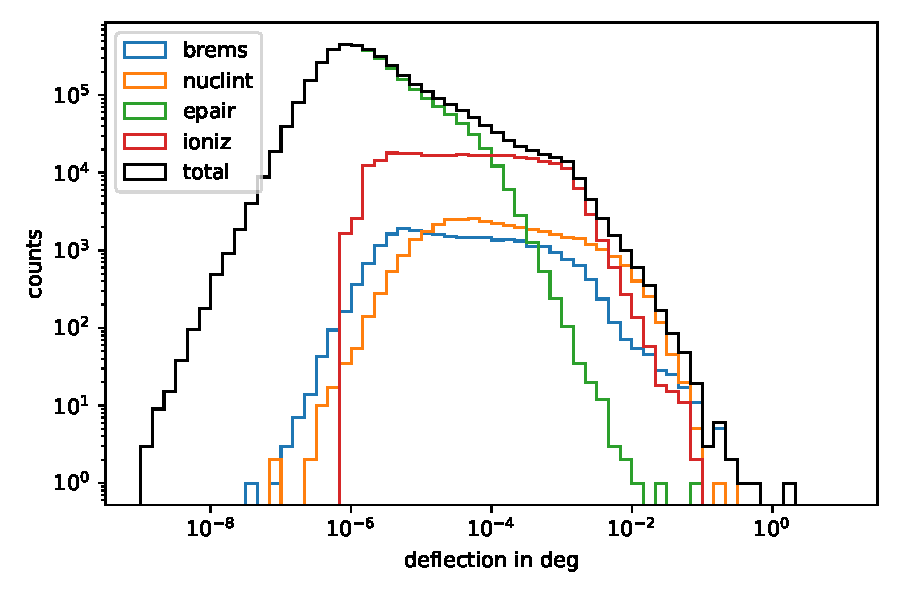
\includegraphics[width=0.8\textwidth]{figures/1PeV_1TeV_1000events.pdf}
    \caption{The propagation is done for $\num{1000}$ 
    muons from $E_{\text{i}} = \SI{1}{\peta\electronvolt}$ to $E_{\text{f,\,min}} = \SI{1}{\tera\electronvolt}$ using $\texttt{e\_cut} = \SI{500}{\mega\electronvolt}$ and $\texttt{v\_cut} = 0.05$. For multiple scattering 
    the Moliére parametrization.}
    \label{fig:defl_per_int}
\end{figure}

